% This file (dissertation-main.tex) is the main file for a dissertation.
\documentclass {udthesis}
% preamble

% Include graphicx package for the example image used
% Use LaTeX->PDF if including graphics such as .jpg, .png or .pdf.
% Use LaTeX->PS->PDF if including graphics such as .ps or .eps
% Best practice to not specify the file extension for included images,
% so when LaTeX is building it will look for the appropriate image type.
\usepackage{graphicx}
\usepackage[acronym]{glossaries}
\usepackage{enumitem}
\usepackage{amsmath}
\usepackage{caption}
\usepackage{subcaption}

%%%%%%%%%%%%%%%%%%%%%%%%%%%%%%%%%%%%%%%%%%%%%%%%%%%%%%%%%%%%
% List of acronyms
%%%%%%%%%%%%%%%%%%%%%%%%%%%%%%%%%%%%%%%%%%%%%%%%%%%%%%%%%%%%

\newacronym{auv}{AUV}{Autonomous Underwater Vehicle}
\newacronym{rov}{ROV}{Remotely Operated Vehicle}
\newacronym{hov}{HOV}{Human Operated Vehicle}
\newacronym{api}{API}{Application Program Interface}
\newacronym{dyi}{DYI}{Do It Yourself}
\newacronym{ros}{ROS}{Robot Operating System}
\newacronym{dof}{DOF}{Degree of Freedom}
\newacronym{imu}{IMU}{Inertial Measurement Unit}
\newacronym{cad}{CAD}{Computer Aided Design}
\newacronym{lipo}{LiPo}{Lithium Polymer}
\newacronym{tcp}{TCP}{Transmission Control Protocol}
\newacronym{acp}{AC}{Alternating Current}
\newacronym{dcp}{DC}{DIrect Current}
\newacronym{fps}{FPS}{Frames Per Second}
\newacronym{ar}{AR}{Augmented Reality}
\newacronym{rst}{RST}{Rotation, Scaling and Translation}
\newacronym{fov}{FOV}{Field of View}



\makeglossaries
\graphicspath{{fig/}}

\begin{document}

%=========================================================================================
% Eigen-value Shape Descriptors

\chapter{Eigen-Value based shape descriptors}
\label{chap:eigen}

%=========================================================================================
% Outlines
%=========================================================================================
% Chap3: Eigen-value descriptors
\section{Outline}
Identification is challenging and tricky; promising solutions can often fail; for example eigen-value based shape descriptors fail to identify objects from noisy image datasets.

\begin{enumerate}[label=Section \arabic*:, start=0]
\item Intro

\item Eigen-value shape descriptors provide a mathematical framework for identifying geometric shapes.

    \begin{enumerate}[label=Para \arabic*:, start=1]
      
	\item Objects characterized by a unique shape that is in contrast with their environment can be identified using shape-based descriptors.
	
	\item In shape-based identification problems, position and orientation of objects could be unknown: descriptors that can identify shapes irrespective of variations in rotation, scaling and translation of objects are useful in such cases.
	
	\item The question ``Can one hear the shape of a drum?'' -Kac, motivated the development of eigen-value based shape descriptors.
	
	\item Eigen-value shape descriptors offer a rotation, scaling and translation invariant framework for identifying geometric shapes.  
	
    \end{enumerate}
    
\item Here is how eigen-value descriptors can be used to recognize objects like subway cars from sonar backscatter images.

    \begin{enumerate}[label=Para \arabic*:, start=1]

      \item Since man-made objects are often produced in strict geometrical shapes when compared with natural objects they can exhibit wide intra and inter species variation, man-made objects can often be identified from natural scenes from their shape alone.
      
      \item Studying the impact to underwater ecosystem of subway cars in the ocean floor along the coast of NY-NJ, is an ongoing research problem.
      
      \item Subway cars in sonar back scatter images can be manually identified from their rectangular shape which contrasts with other objects in the ocean floor.
      
    \end{enumerate}

\item The rotation, scaling and translation (RST) invariance properties offered by the eigen-value descriptors is shown to be adversely affected by image noise and signal discretization.

    \begin{enumerate}[label=Para \arabic*:, start=1]

      \item The RST invariance properties and shape recognition performance of eigen-value shape descriptors is severely affected by noise.
      
      \item The RST invariance properties of eigen-value descriptors theoretically defined over a continuous domain can be adversely affected by the discretization errors introduced in the computation process. 
      
    \end{enumerate}

\item The Eigen-value descriptors, though effective in recognizing simple shapes in the absence of noise, cannot handle complex objects corrupted by noise or objects characterized by textural features.

    \begin{enumerate}[label=Para \arabic*:, start=1]

      \item Objects that require more than shape features, for example texture, cannot be identified using eigen-value shape descriptors.
      
      \item Objects corrupted by noise could adversely affect the performance of eigen-value shape descriptors.
      
    \end{enumerate}
    
\end{enumerate}

%=========================================================================================

\section{Introduction}

Identification of objects is a challenging and tricky problem. One way to recognize objects is through shape identification \cite{shape_survey}. Eigen-value based shape descriptors \cite{khabou,zuliani}, is a mathematical framework that can identify prespecified geometric shapes in images. This method can be used to detect artificially introduced man-made objects describable by a strict geometric shape amongst other naturally occurring objects in images. An application for such a shape identification method was identified in the Redbird reef site. In the Redbird reef site off the coast of New York-New Jersey, subway cars were dropped into the sea to aid artificial reef development \cite{redbird1, redbird2}. When research studies were conducted to study the impact of these subway cars on the geologic features \cite{redbird_nicole, redbird_art}, the need for an automated method to pinpoint the 
locations of artificial objects 
from sonar survey data became apparent. Eigen-value shape descriptors were employed to solve this problem.


\section{Background}

Eigen-value based shape descriptors is an object recognition solution designed to identify objects characterized by a specific shape. Additionally, eigen-value shape descriptors require the object that is to be detected to have a unique prespecified shape that contrasts with the other objects found in the environment. This requirement is readily met when trying to identify man-made objects form natural scenes. Man-made objects tend to have strict geometric shapes compared to naturally occurring objects which exhibit a wide variation in shape and appearance. This suggests that eigen-value shape descriptors may be a useful tool for recognizing specific objects from natural images.

In shape-based identification problems, even if prior knowledge is available about the shape of the objects, the position and orientation of objects could be unknown. The task of searching for the same shape over different orientations in an image makes it computationally intensive. It is more effective to have a solution that can identify shapes irrespective of variations in rotation, scaling and translation of objects or in other words use a shape descriptor that is \gls{rst} \textit{invariant}. The \gls{rst}-invariant nature of eigen-value shape descriptors makes it a useful tool for object recognition. 

``Can one \emph{hear} the shape of the drum?'' This famous question by Kac \cite{kac} laid the foundation for the research into eigen-value shape descriptors.
This question can be rephrased as ``Can one determine the shape of the drum membrane from the principal modes of vibration of the sound it produces?''.
If the principle modes of vibration of each drum membrane shape were unique, then would be an appealing possibility of using the eigen modes as descriptors for shape of drum membranes. 
Through a later work, Gordan et.al.\cite{gordon} proved that a pair of iso-spectral drums produce sound with same principal modes. The work by Gorden answers Kac's question by stating that the eigen modes are not sufficient to uniquely identify the shape of a drum. However two independent papers by Khabou and Zuliani \cite{khabou,zuliani} show that eigen modes can still be used as shape descriptors for practical purposes.

Eigen-value based shape descriptors offer a \gls{rst} invariant object recognition solution for identifying predefined shapes. This is useful in applications where the objects to be recognized can be distinguished from other background objects primarily using their shape. This property is especially useful for identifying artificial objects with a well defined shape from natural scenes.


\section{Preliminaries}

The mathematical formulation of identifying the bounded planar domain $\Omega$ from its eigen-values $\lambda_{i}$ can be applied to object recognition problems \cite{khabou, zuliani}. The $\lambda_{i}$'s are the eigen-values of the helmholtz differential equation \eqref{eq:helmholtz} with Dirichlet boundary condition $u=0$ on the boundary of the domain $\delta\Omega$.
%
\begin{equation} \label{eq:helmholtz}
\Delta u+\lambda u = 0
\end{equation}
%
When cast as an object to be recognized, the domain $\Omega$ is a binary profile representation of a shape in an image.
Let the sequence of computed eigenvalues $\lambda_i$ be
%
\begin{equation} \label{eq:eigenvalue}
0<\lambda_{1}\leq\lambda_{2}\leq\lambda_{3}\leq\dots\leq\lambda_{k}\leq\dots\rightarrow\infty.
\end{equation}
%
A shape $\Omega$ can then be represented as a finite $n$-element vector of eigen ratios, which we call as shape descriptor $F$. For this application, the length of shape descriptor was truncated to 17 ($n=17$).
%
\begin{equation} \label{eq:eigenratio}
F(\Omega) = \left\{\frac{\lambda_{1}}{\lambda_{2}},\frac{\lambda_{1}}{\lambda_{3}},\frac{\lambda_{1}}{\lambda_{4}},\dots,\frac{\lambda_{1}}{\lambda_{n}}\right\}.
\end{equation}
%
The angle $\Theta$ between two shape descriptor vectors $F(\Omega_{1})$ and $F(\Omega_{2})$ can be used as relative a measure of dissimilarity between the two shapes $\Omega_{1}$ and $\Omega_{2}$,
%
\begin{equation} \label{eq:eigendist}
\Theta\left(\Omega_{1},\Omega_{2}\right)=\cos^{-1}\left(\frac{\langle F(\Omega_{1}),F(\Omega_{2})\rangle}{\|F(\Omega_{1})\|\|F(\Omega_{2})\|}\right).
\end{equation}
%
Small values for the angle $\Theta$  would imply that the two shapes $\Omega_{1}$ and $\Omega_{2}$ are similar.
For a pair of objects whose $\Theta$ value is less than a threshold, 
we can assume that the two objects are identical in terms of their shape.


\section{Subway-car Detection from Seabed Images} \label{sec:subwaycar_results}


The ability of eigen-value shape descriptors to match to certain shapes can be used for object recognition in natural images, especially for identification of artificial objects from natural scenes. Artificial, or \textit{man-made}, objects are often characterizable by a prespecified shape. On the other hand, naturally occurring objects can exhibit wide intra-species and inter-species variation. For instance, it is easier to define the shape of an artificial object like a book compared to a natural object like a leaf. This enables eigen-value shape descriptors to pick out artificial objects from natural scenes based on their shape alone.

This problem of recognizing artificial objects from natural scenes was encountered while marine geologists were studying the Redbird artificial reef site \cite{redbird_nicole, redbird_art}. The focus of these studies were to observe geologic sub-sea features around artificial objects like subway cars. An automated method to detect subway cars would significantly facilitate such studies. 

\begin{figure}
  \begin{subfigure}[]{0.9\textwidth}
      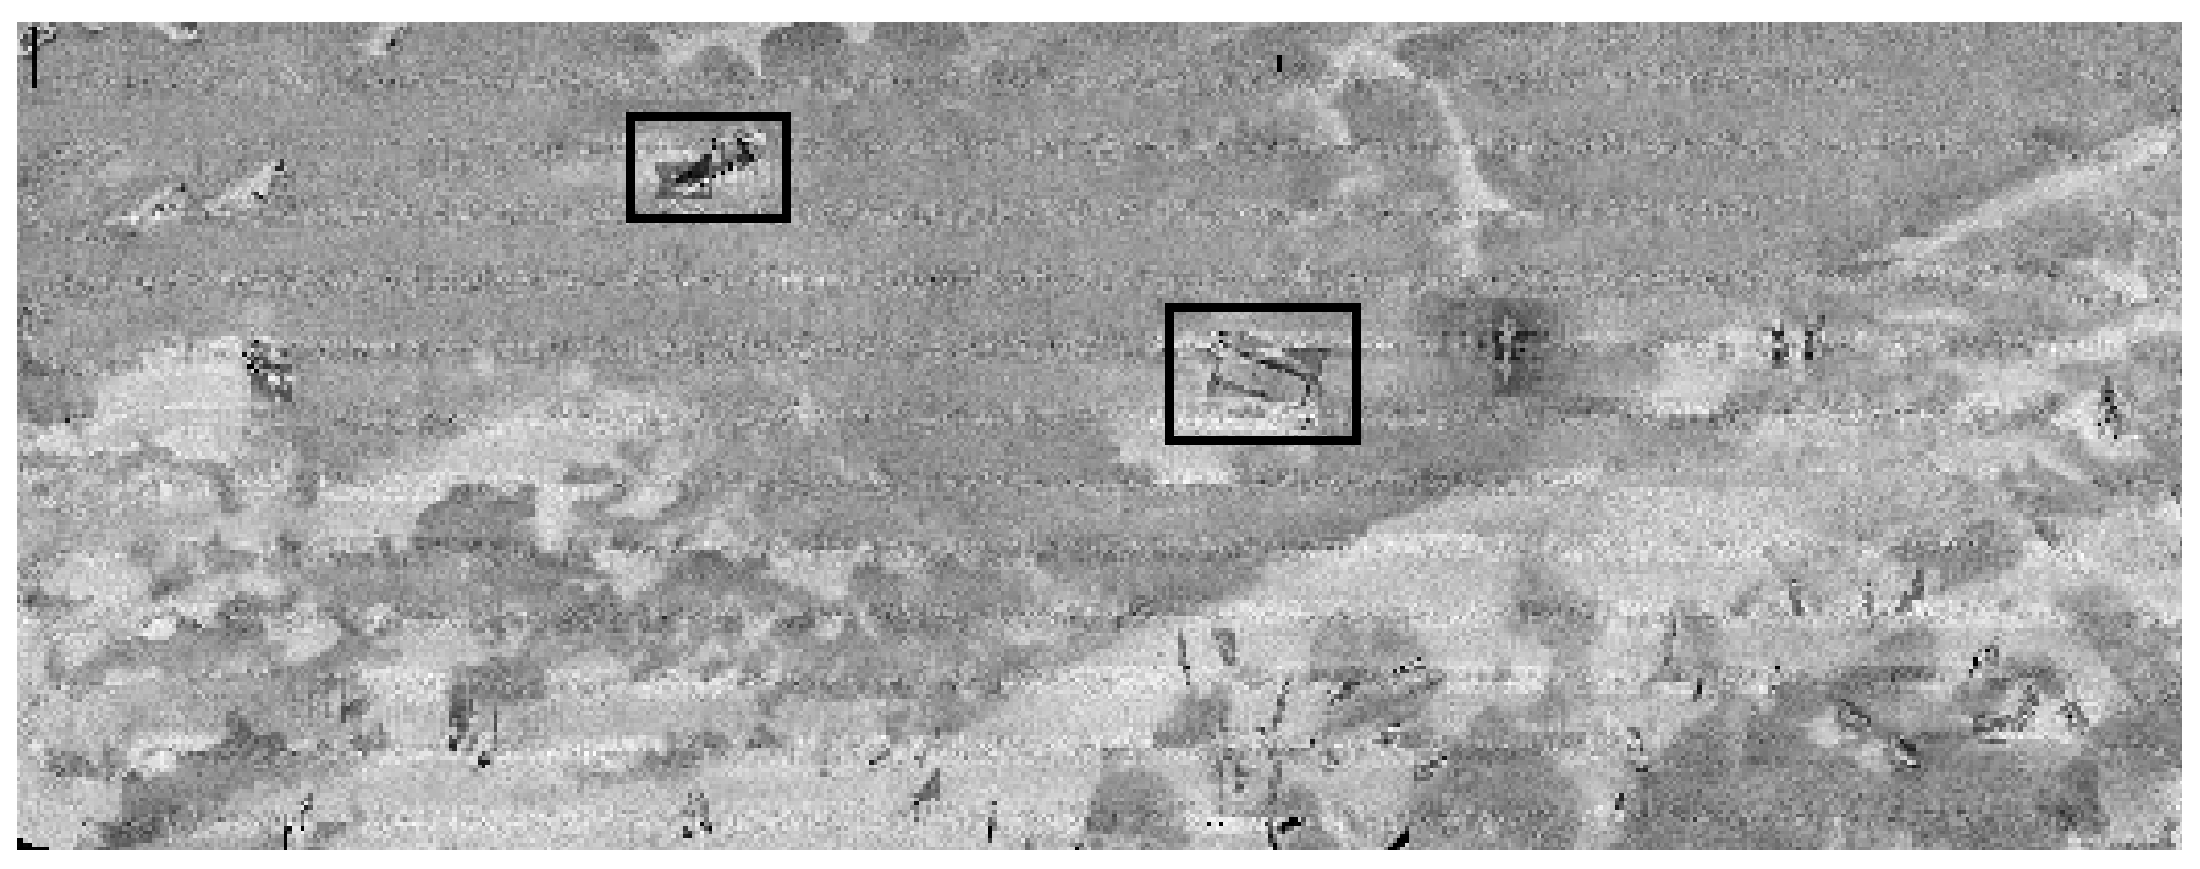
\includegraphics[width=\textwidth]{subwayorig}
      \caption{Backscatter image of sea-floor from Gavia AUV}
      \label{subfig:subwayorig}
  \end{subfigure}
  \begin{subfigure}[]{0.9\textwidth}
      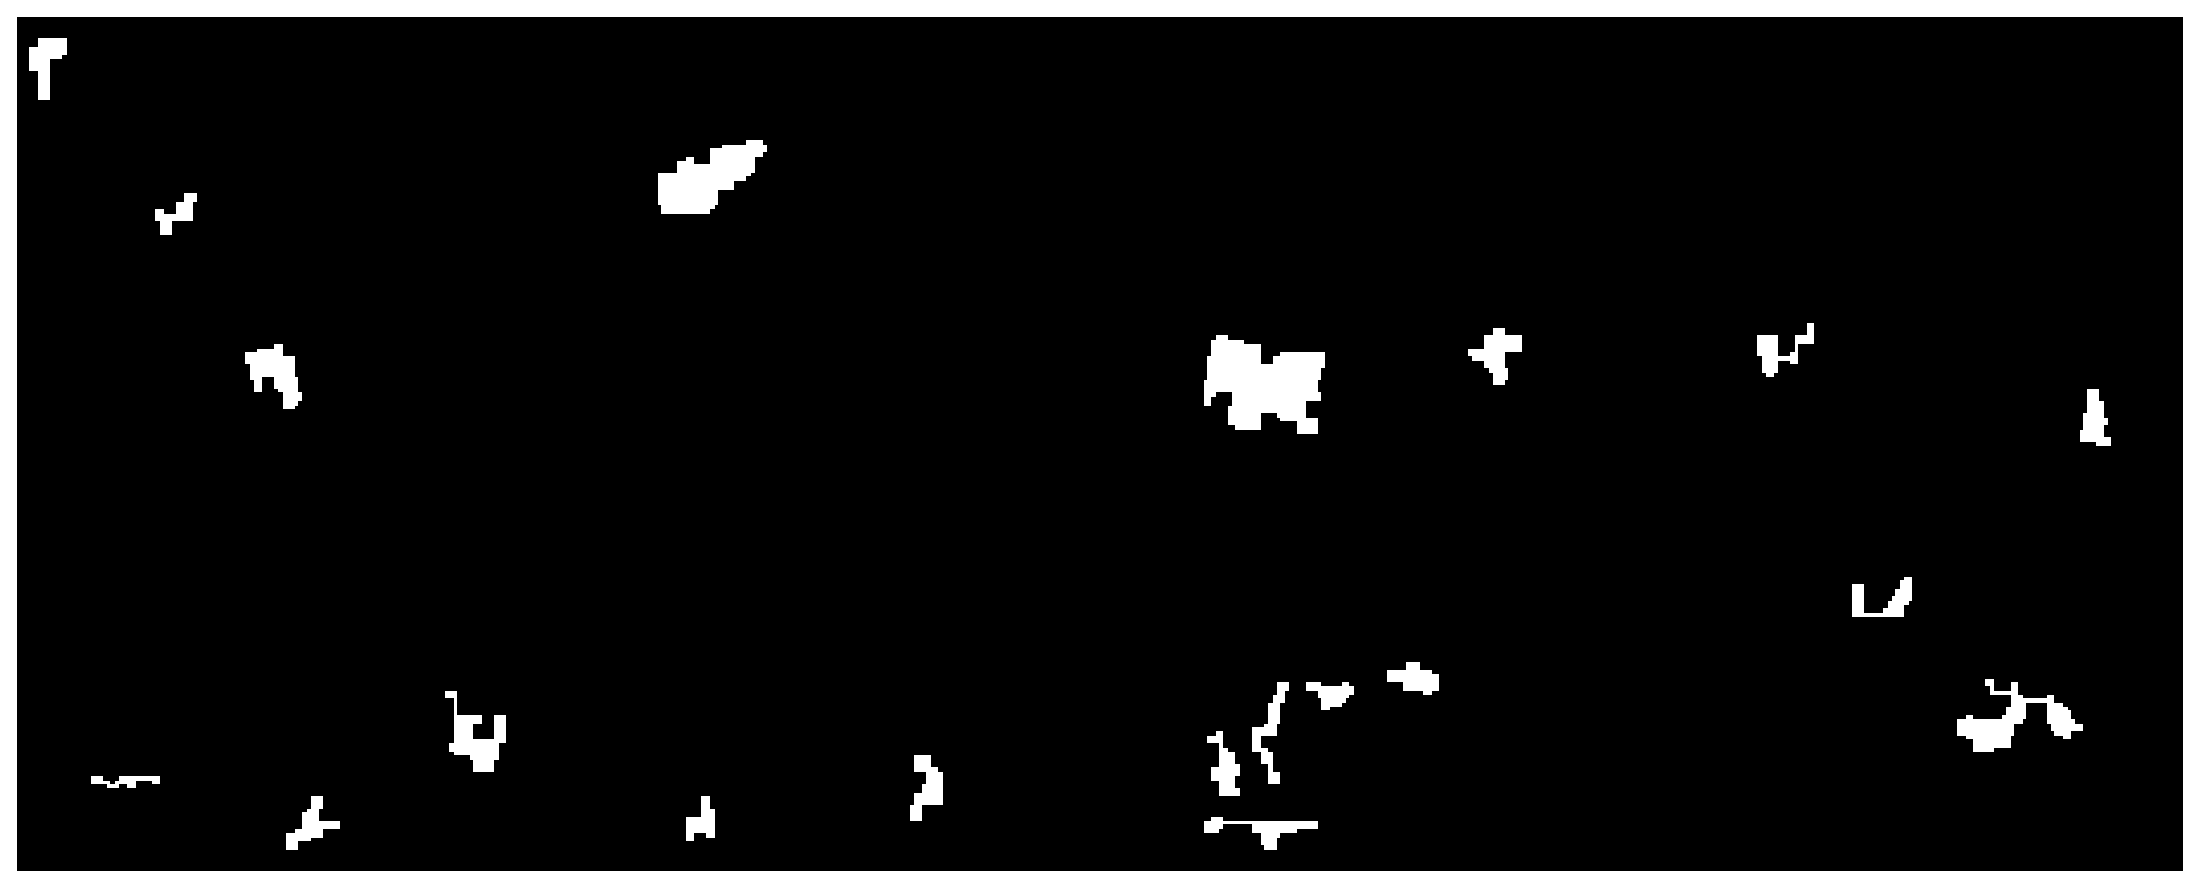
\includegraphics[width=\textwidth]{subwaysegment}
      \caption{Image segmentation using basic morphological operations and edge detection}
      \label{subfig:subwaysegment}
  \end{subfigure}
\caption[Analysis of sonar backscatter image of Redbird reef]{}
\end{figure}

The sonar backscatter image of Redbird reef in Figure~\ref{subfig:subwayorig} shows the shape profiles of some sunken objects resting on the seabed. Two subway cars are marked using black rectangles. If we look for rectangular objects like the rectangle in Figure~\ref{subfig:subwayrect}, it is likely that eigen-value shape descriptors will distinguish the profiles of subway-cars, as there are no other objects with such rectangular shape profile in the seabed image (Figure~\ref{subfig:subwayorig}). 

\begin{figure}
    \centering      
    
\includegraphics[width=0.4\textwidth]{eigenrect}
    \caption[Rectangular template used as reference shape for subway-cars]{Rectangular template used as reference shape for subway-cars}
    \label{subfig:subwayrect}
\end{figure}
%
\begin{figure}
    \centering
    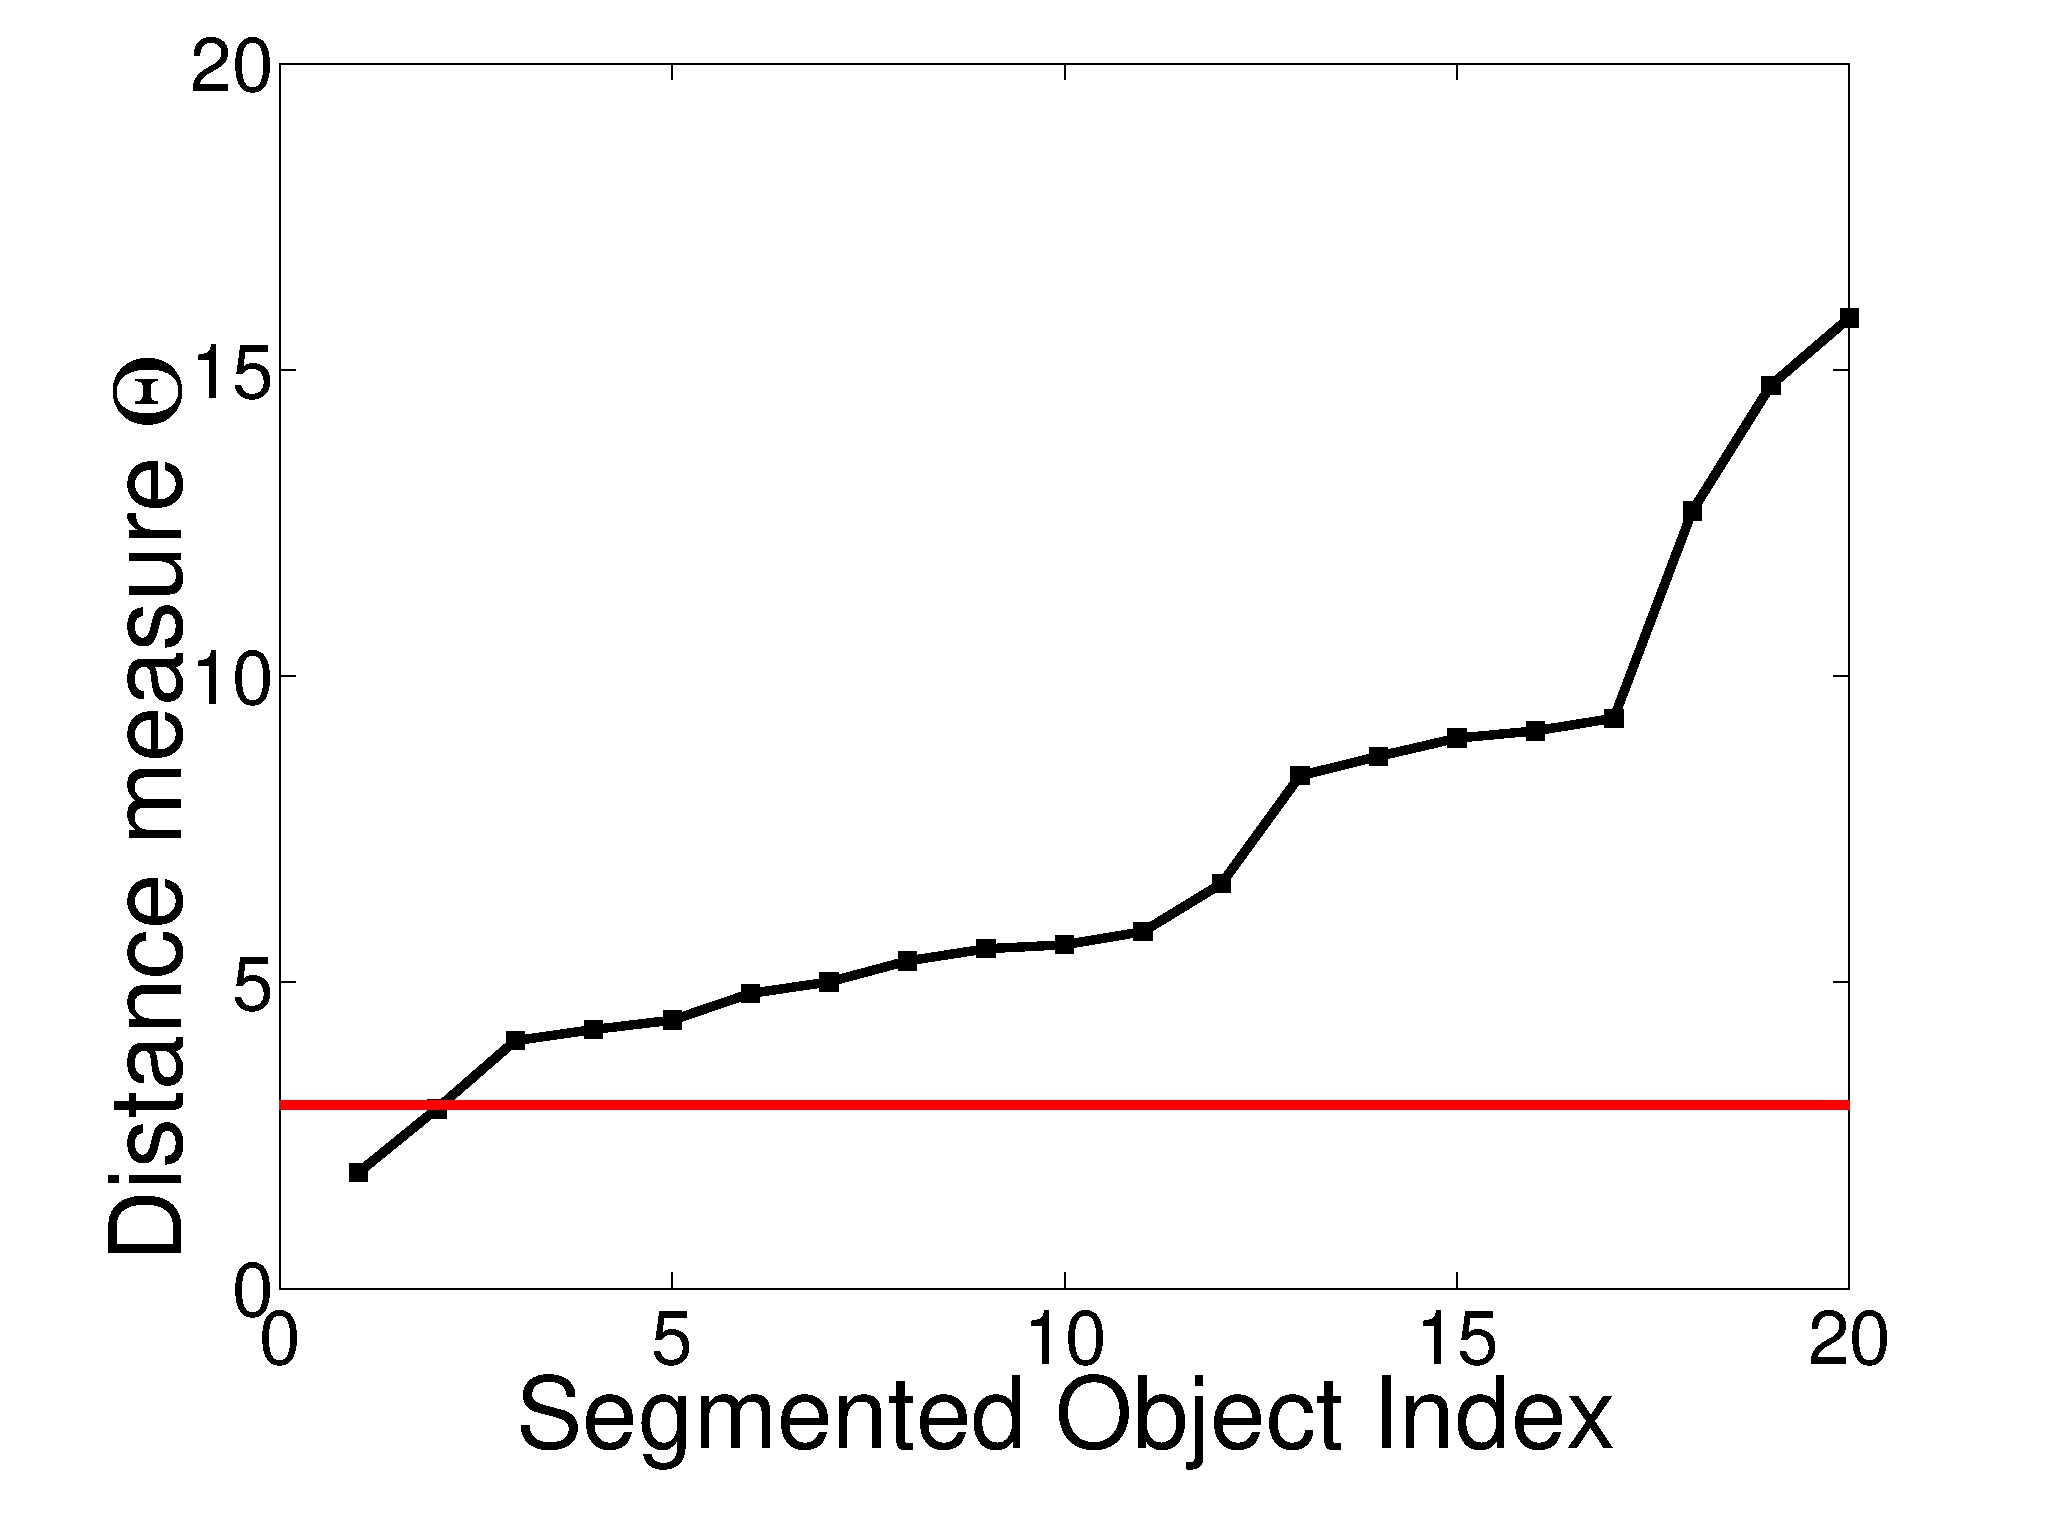
\includegraphics[width=0.8\textwidth]{subway_dot_prod}
    \caption[Plot of similarity measures of different underwater objects to the subway car reference profile]{Plot of the weighted distance D between each segmented feature and the template rectangle in Figure~\ref{subfig:subwayrect}. The threshold (D=3) is shown as a red line.}
    \label{subfig:eigendistances}
\end{figure}

In order to verify the ability of eigen-value shape descriptors to pick out the subway-cars in Figure~\ref{subfig:subwayorig}, we follow a sequence of steps. The sonar backscatter image is first segmented to get a series of shape profiles using a grayscale threshold operation on the image. Figure~\ref{subfig:subwaysegment} shows the different ``blobs'' obtained after thresholding. The blobs were then compared to the rectangular shape in Figure~\ref{subfig:subwayrect} using the angle $\Theta$ metric that was defined in \eqref{eq:eigendist}. The $\Theta$ value of a blob is a direct indicator on how close in appearance it is to the reference rectangle in Figure~\ref{subfig:subwayrect}. The smaller the $\Theta$ value, the closer it is in appearance to the reference rectangle shape $\Omega_r$. The $\Theta(\Omega_r,\Omega_j)$ value for each blob $j$ is recorded and the $\Theta$ values are plotted in ascending order in Figure~\ref{subfig:eigendistances}. 

The two blobs that correspond to subway cars have the lowest $\Theta$ values. The blob with the lowest $\Theta$ value ($\Theta=1.89^{\circ}$) along with its plotted shape descriptor $F$ is shown in Figure~\ref{subfig:subwaybest1}. Similarly the blob with the second lowest $\Theta$ value is shown in Figure~\ref{subfig:subwaybest2}($\Theta=2.93^{\circ}$). In Figures~\ref{subfig:subwaybest1} and ~\ref{subfig:subwaybest2}, the blue line corresponds to the shape descriptor $F(\Omega_r)$ of reference rectangle $\Omega_r$ and the red line corresponds to the shape descriptor $F(\Omega_j)$ of blob $j$. The $\Theta(\Omega_r,\Omega_j)$ is the computed angle between the shape descriptor vectors as discussed in \eqref{eq:eigendist}. In contrast, the blob with the largest $\Theta$ value ($\Theta=15.85^{\circ}$) or in other words the blob that matches the least with the reference rectangle is shown in Figure~\ref{subfig:subwayworst}. In this case, if we set a threshold $\Theta_{thresh}=3$ and only consider objects with $\
Theta<\Theta_{thresh}$ to 
be subway cars, then we have a mechanism to detect subway cars from other objects present in this sonar image. This effectively shows that eigen-value shape descriptors are in principle capable of picking up prespecified shapes from images.

\begin{figure} 
  \centering
  \begin{subfigure}[]{0.45\textwidth}
      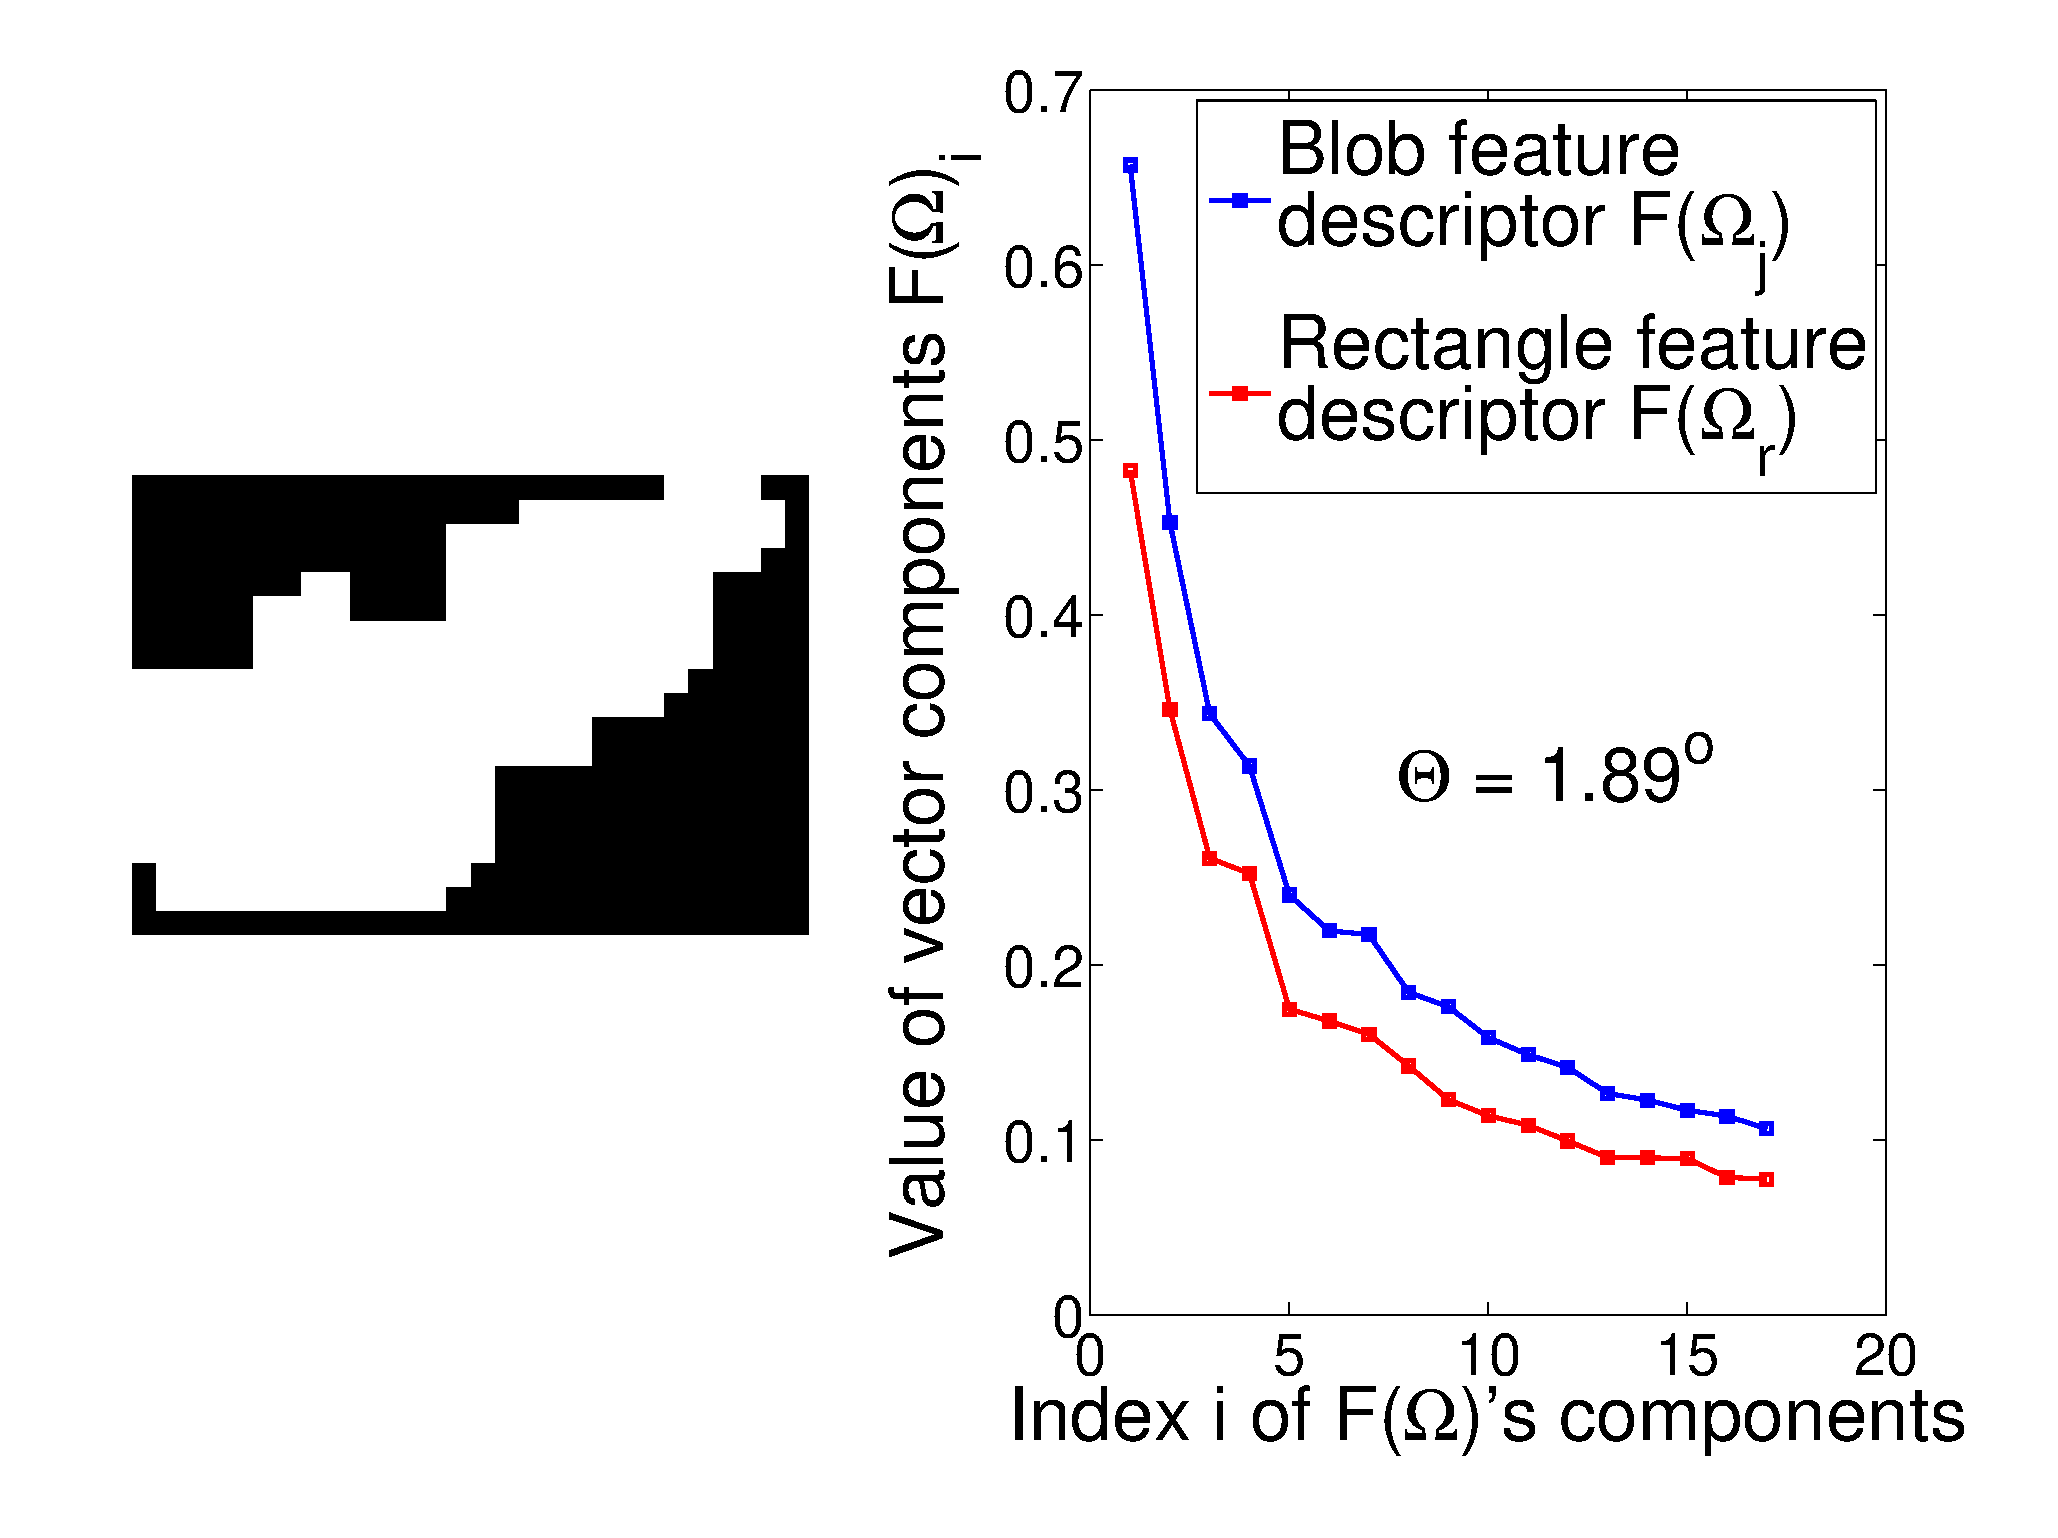
\includegraphics[width=\textwidth]{best1}
      \caption{}
      \label{subfig:subwaybest1}
  \end{subfigure}
  \begin{subfigure}[]{0.45\textwidth}
      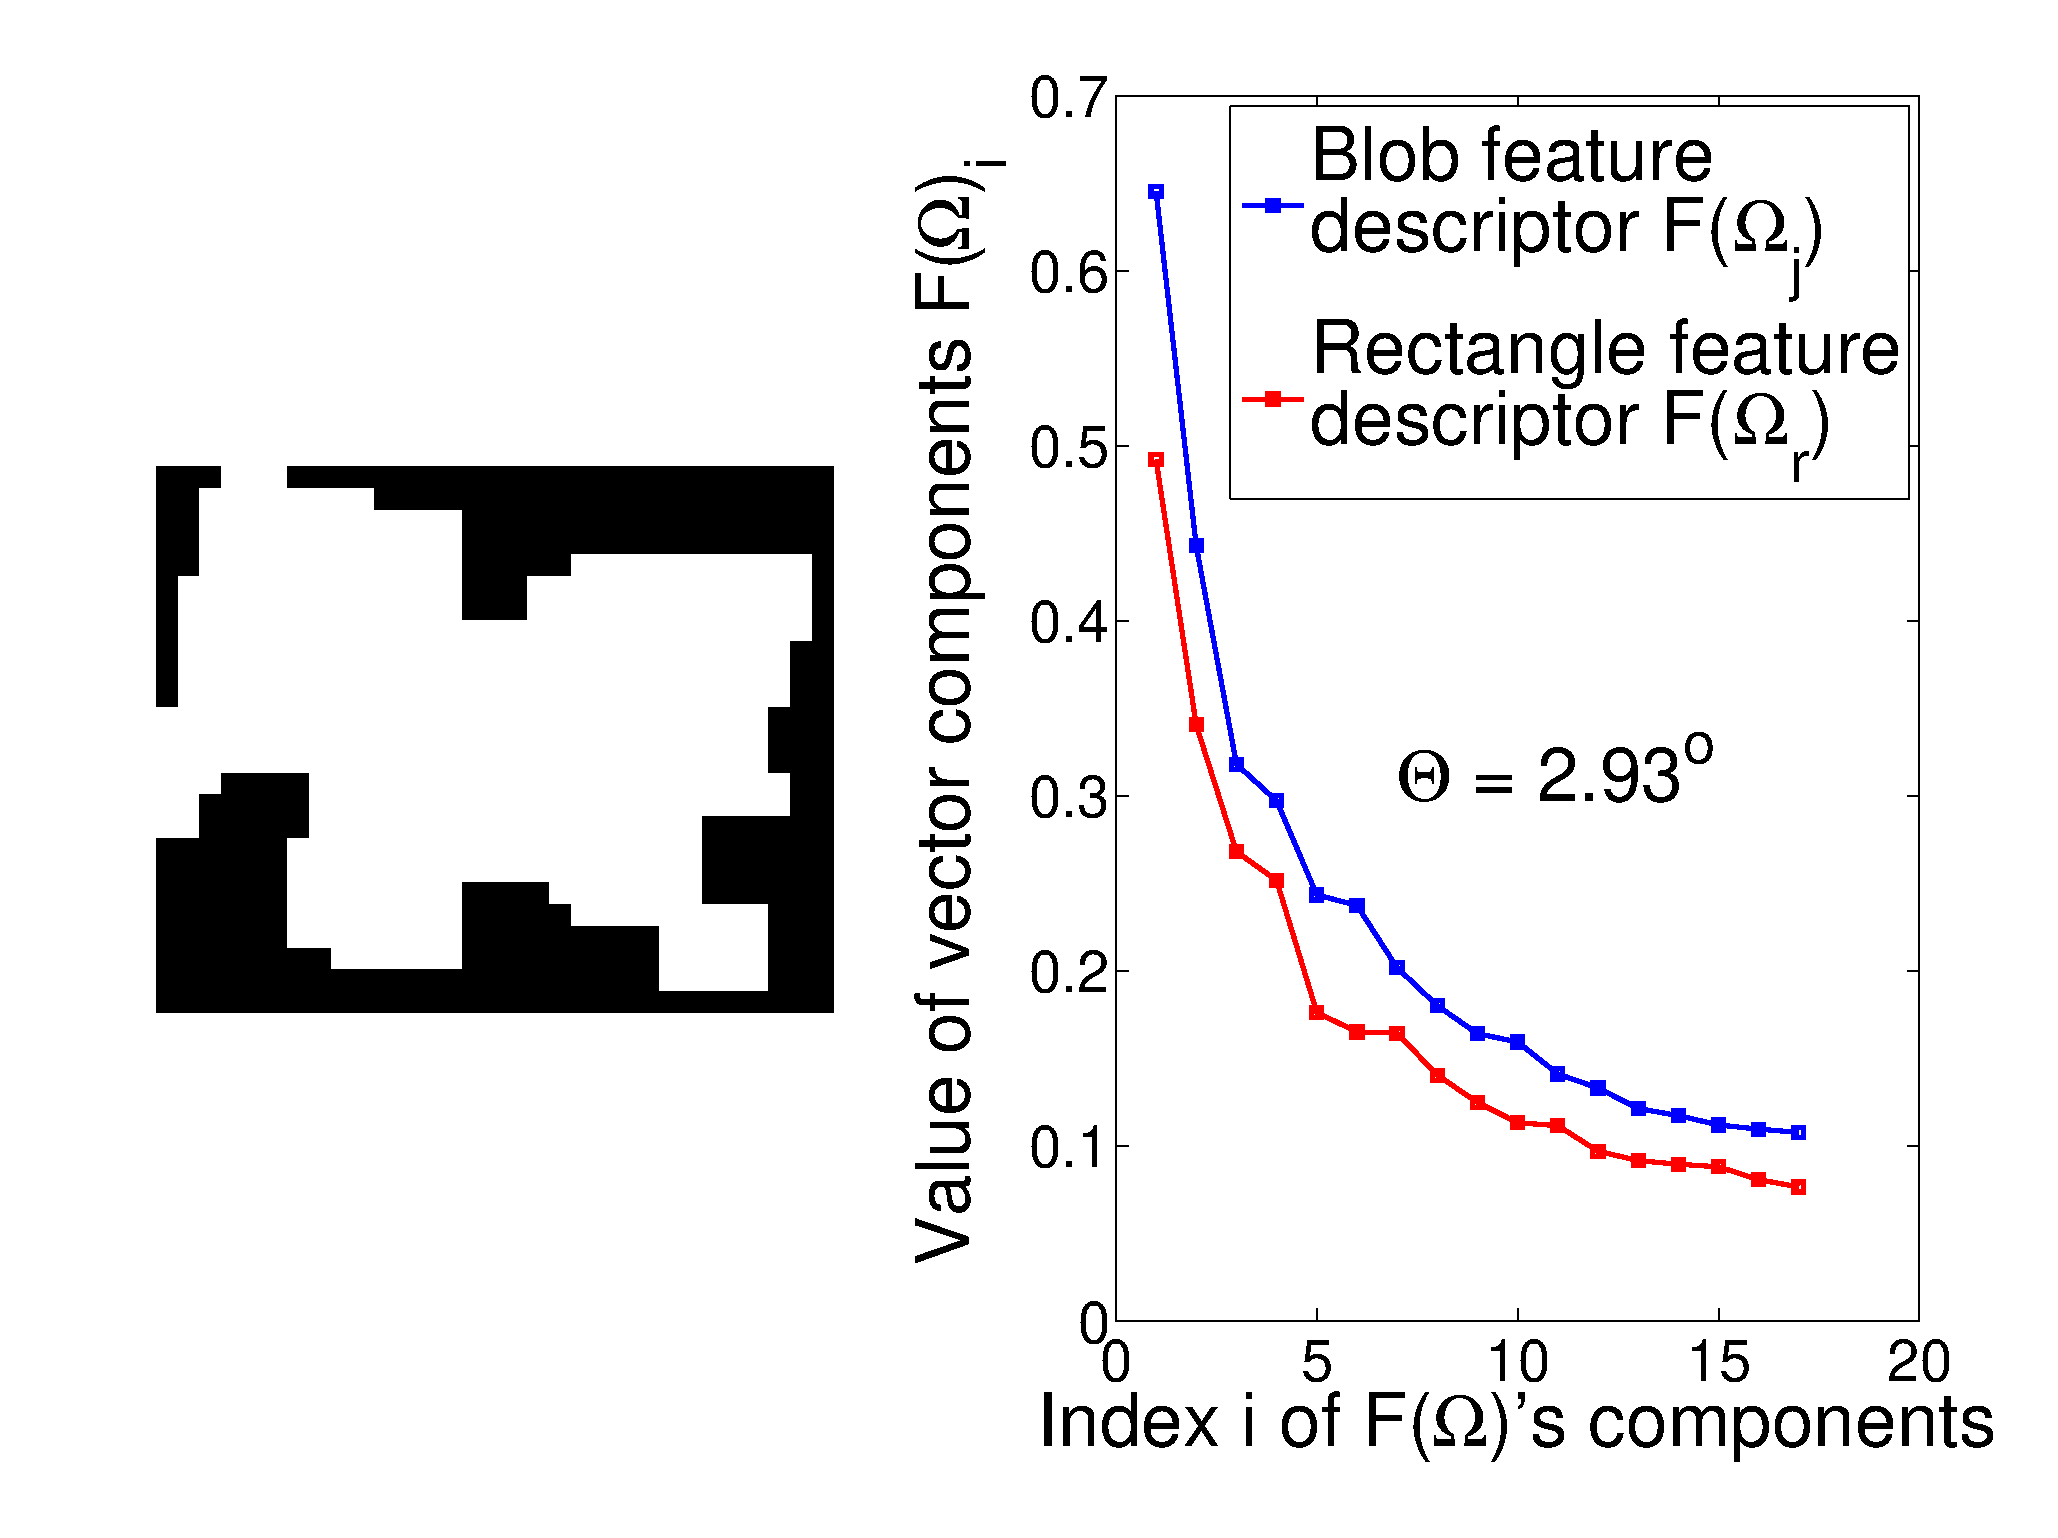
\includegraphics[width=\textwidth]{best2}
      \caption{}
      \label{subfig:subwaybest2}
  \end{subfigure}
  \begin{subfigure}[]{0.45\textwidth}
      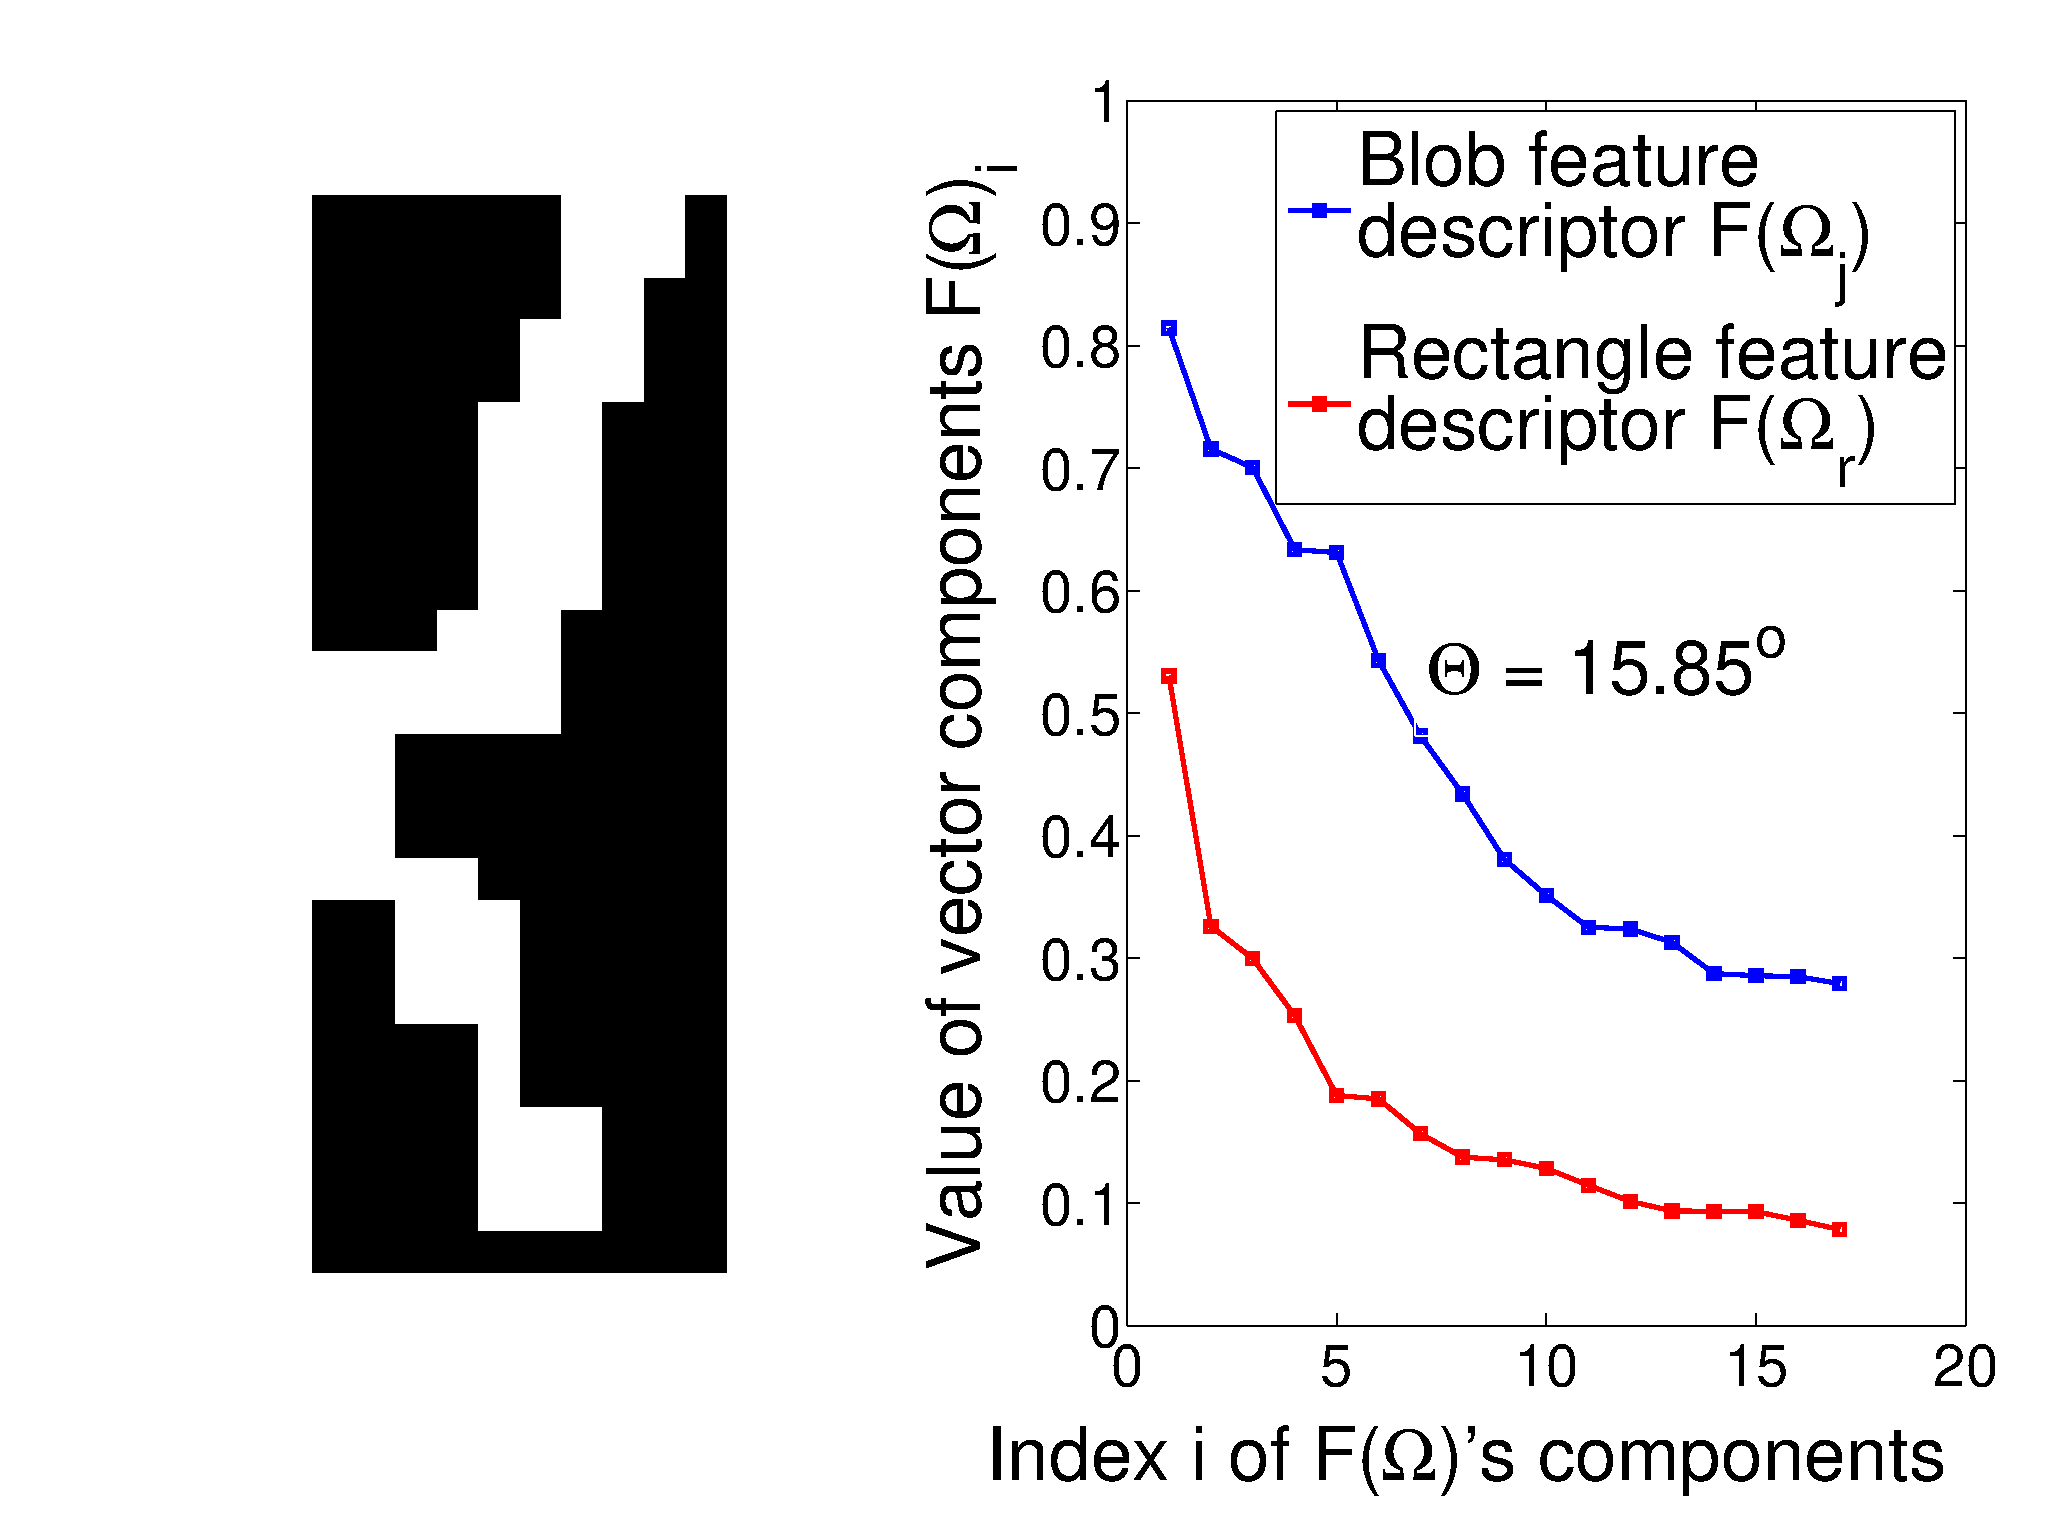
\includegraphics[width=\textwidth]{worst1}
      \caption{}
      \label{subfig:subwayworst}
  \end{subfigure}
\caption[Subway car recognition results]{Parts (\subref{subfig:subwaybest1}) and (\subref{subfig:subwaybest2}) correspond to the blobs that are closest to the reference rectangle in Figure~\ref{subfig:subwayrect}. The shape of the blob $j$ is shown on left and the corresponding plot of shape descriptor $F(\Omega_j)$ (red line) along with the plot of the reference rectangular profile (blue line) is shown on right. The distance measure $\Theta$ between the blob and the reference rectangle gives a picture of how close the given blob is to the reference rectangle. A contrasting view of the blob that matches the least with the reference rectangle is shown in (\subref{subfig:subwayworst}).}
\end{figure}      


\section{Discussion}

In Section~\ref{sec:subwaycar_results}, we saw how eigen-value shape descriptors can be utilized to detect subway cars from other underwater objects. The eigen-value shape descriptors here were tuned to look for rectangular objects that match the profile in Figure~\ref{subfig:subwayrect}. The blobs obtained as matches to the reference rectangle through this eigen-value shape descriptor method complies with the ground truth information on the position of the subway cars in the sonar image (Figure~\ref{subfig:subwayorig}). Hence from this study, we see that eigen-value shape descriptors provide a viable mechanism to detect objects with specific shapes.

Since eigen-value shape descriptors purely rely on the shape of an object, two objects with identical shapes but significantly different textures cannot be differentiated using this method. In tests we performed, eigen-value descriptor did not perform well on objects whose shape is characterized by more complex contours. For instance when eigen-value shape descriptors were evaluated as a tool to recognize numbers between 0 and 9, 1 and 7 were often confused and wrongly classified. Similar misclassifications were also registered between 0,6,8 and 9. These errors can be attributed to the \gls{rst} invariance property coupled with discretization errors while representing numbers (0-9) in an image form. Even though \gls{rst} invariance is helpful in some cases, it can be detrimental when the orientation of a shape can play a part in the recognition process. The theoretical mechanism behind the eigen-value shape descriptors defines it over a continuous domain. When eigen-value shape descriptors were adopted as a 
shape 
identification tool on images, the domain needed to be discretized; images are nothing but discrete spatial arrangement of pixel values. When dealing with complex shapes, there can be significant discretization errors that can adversely affect the performance of eigen-value shape descriptors. High levels of noise and errors in segmentation are other significant factors that can lower the performance of eigen-value shape descriptors.


\section{Conclusion}

Eigen-value based shape identification is a tool that can be used to identify simple predefined shapes from natural images. This method was successful in identifying subway-cars from sonar images of the seabed under the assumption that subway cars are rectangular in shape. Apart from shape, the texture of an object plays a key role in determining the identity of an object. Since eigen-value shape descriptors discard textural information, they are not suited for applications where shape is insufficient to decipher the identity of an object. Additionally, while dealing with complex shapes, there can be significant discretization error, and also segmentation errors which can affect the shape profile of an object. Such errors often diminish the performance of eigen-value shape descriptors. Hence eigen-value shape descriptors is a useful tool for identifying objects provided we can guarantee that the shape of the object can be described in a discrete domain with minimal error. Furthermore, for this method to work,
 the 
objects we are interested in should exhibit a shape profile that is significantly different from all other objects in the background. 

Natural objects, like marine organisms, are typically associated with complex shape profiles. Furthermore texture is often a key discriminant required to identify marine organisms. The inability to use textural information, among other factors, limits eigen-value shape descriptors to few specialized object recognition applications only. Chapter~\ref{chap:scallop_recog} offers a multi-layered object recognition solution that attempts to overcome some drawbacks seen in eigen-value shape descriptor approach.

%========================================================================================
\printglossary[type=\acronymtype]                  
%
% This is the Bibliography file (bibtex.tex)
% This generally works for BibTeX

% Use sample.bib for BibTeX database
\bibliography{thesis_ref}
% BibTeX style (plain, alpha, unsrt)
\bibliographystyle{plain}
   % This file (bibtex.tex) contains the text
                   % for a bibliography if using BibTeX with
                   % sample.bib
\end{document}


